\documentclass{cubeamer}

\usepackage{graphicx}
\usepackage{caption}
\usepackage{subcaption}
\captionsetup[figure]{font=tiny,skip=0pt}
\captionsetup[subfigure]{font=tiny,skip=-3pt}
\captionsetup[sub]{font=small,skip=0pt}
% \usepackage{subcaption}

\usepackage[sfdefault]{FiraSans}
\setsansfont[
  BoldFont={Fira Sans SemiBold},
  ItalicFont={Fira Sans Italic},
  BoldItalicFont={Fira Sans SemiBold Italic}
]{Fira Sans}

\usepackage{subfiles}
\usepackage{tikz}
\usetikzlibrary{arrows,shapes,3d,positioning}
\usepackage{import}
\subimport{layers}{init}

% math stuff
\usepackage{amsmath}                % to use DeclareMathOperator
\usepackage{amssymb}
\usepackage{mathrsfs}
\usepackage{mathtools}
\usepackage{xargs}                  % for more than one optional arguments when define new commands
\usepackage{physics}                % vectors
\usepackage{mdframed}               % frames for definition, theorem, etc.
\usepackage[ruled]{algorithm2e}     % for algorithms
\usepackage{ifthen}                % for \ifthenelse
\usepackage{upgreek}

% formatting some important single letters
\renewcommand{\epsilon}{\varepsilon}
\renewcommand{\phi}{\varphi}
\renewcommand{\upepsilon}{\upvarepsilon}
\renewcommand{\upphi}{\upvarphi}

% new operators
\DeclareMathOperator*{\argmin}{arg\,min}                % argmin
\DeclareMathOperator*{\argmax}{arg\,max}                % argmax
\DeclarePairedDelimiter\ceil{\lceil}{\rceil}            % ceiling function
\DeclarePairedDelimiter\floor{\lfloor}{\rfloor}         % floor function
\DeclarePairedDelimiter{\parens}{\lparen}{\rparen}      % parenthesis (use \parens* for automatically adjusting version)
\DeclarePairedDelimiter{\bracket}{[}{]}
\DeclarePairedDelimiter{\cbracket}{\{}{\}}
% \DeclarePairedDelimiter{\fourier}{\mathscr{F}\{}{\}}
% \DeclarePairedDelimiter{\invfourier}{\mathscr{F}^{-1}\{}{\}}

\newcommand{\fourier}[1]{\mathscr{F}\cbracket*{#1}}
\newcommand{\invfourier}[1]{\mathscr{F}^{-1}\cbracket*{#1}}
\newcommand {\dx}{\,dx}
\newcommand {\dy}{\,dy}
\newcommand {\dz}{\,dz}
\newcommand {\dt}{\,dt}
\newcommand {\du}{\,du}
\newcommand {\dtheta}{\,d\theta}
\newcommand {\domega}{\,d\omega}



\newcommand{\bigo}[1]{\ensuremath{\mathcal{O}\parens*{#1}}}
% new commands
\newcommand{\st}{such that }
\newcommand{\w}{where }
\newcommand{\del}{\nabla}
\newcommand{\larrow}{\leftarrow}
\newcommand{\rarrow}{\rightarrow}
\newcommand{\tbf}{\textbf}
\newcommand{\tit}{\textit}
\newcommand{\col}{\operatorname{col}}
\newcommand{\mat}[1]{\begin{matrix} #1 \end{matrix}}
% \newcommand{\vect}[1]{\boldsymbol{\mathbf{#1}}}
\newcommand{\vf}[1]{\boldsymbol{\mathbf{#1}}}
\newcommandx*{\seq}[2][1,2]{\ensuremath{#1, \ldots, #2}}
\newcommandx*{\ssum}[3][1,2,3]{\ensuremath{\sum_{#1 = #2}^{#3}}}
\newcommandx*{\sint}[2][1,2]{\ensuremath{\int_{#1}^{#2}}}
% \newcommandx*{\func}[4][1,2,3,4]{\ensuremath{#1^{\parens{#2}}_{#3}\parens{#4}}}
% \newcommandx*{\val}[3][1,2,3]{\ensuremath{#1^{\parens{#2}}_{#3}}}

% \newcommandx*{\func}[4][1=f,2=x,3,4, usedefault]{
%     \ifthenelse{\equal{#3}{}}{\ensuremath{#1_{#4}\parens{\vf{#2}}}}{\ensuremath{#1^{\parens{#3}}_{#4}\parens{\vf{#2}}}}
% }
\newcommandx*{\func}[3][1=f,2,3, usedefault]{
    \ifthenelse{\equal{#2}{}}{\ensuremath{#1_{#3}}}{\ensuremath{#1^{\parens{#2}}_{#3}}}
}
\newcommandx*{\val}[3][1,2,3, usedefault]{
    \ifthenelse{\equal{#2}{}}{\ensuremath{\vf{#1}_{#3}}}{\ensuremath{\vf{#1}^{\parens{#2}}_{#3}}}
}

\newcommandx*{\Expect}[1][1, usedefault]{\ensuremath{\mathbb{E}_{#1}}}  
\newcommandx*{\Real}[1][1, usedefault]{\ensuremath{\mathbb{R}^{#1}}}                % set of real number
\newcommandx*{\Int}[1][1, usedefault]{\ensuremath{\mathbb{Z}^{#1}}}                 % set of integer
\newcommandx*{\Natural}[1][1, usedefault]{\ensuremath{\mathbb{N}^{#1}}}             % set of natural number
\newcommandx*{\normal}[2][1=0, 2=1, usedefault=!]{\ensuremath{\mathcal{N}(#1,#2)}}  % Gaussian distribution

% define frame environment
% \newmdtheoremenv{definition}{Definition}
% \newmdtheoremenv{proposition}{Proposition}
% \newmdtheoremenv{corollary}{Corollary}
% \newmdtheoremenv{lemma}{Lemma}
% \newmdtheoremenv{theorem}{Theorem}
% \newmdtheoremenv{remark}{Remark}

% define keywords for algorithm
\SetKwInOut{Input}{Input}
\SetKwInOut{Output}{Output}
\SetKwInOut{Parameter}{Parameter}

% \begin{theorem}{text}{label}
% refer as \ref{tha:label}

% equation numbering
\numberwithin{equation}{section}

%%%%%%%%%%%%%%%%%%%%%%%%%%%
\usepackage{listings}
\usepackage{xcolor}

\definecolor{codegreen}{rgb}{0,0.6,0}
\definecolor{codegray}{rgb}{0.5,0.5,0.5}
\definecolor{codepurple}{rgb}{0.58,0,0.82}
\definecolor{backcolour}{rgb}{0.95,0.95,0.92}

\lstdefinestyle{mystyle}{
    backgroundcolor=\color{backcolour},   
    commentstyle=\color{codegreen},
    keywordstyle=\color{magenta},
    numberstyle=\tiny\color{codegray},
    stringstyle=\color{codepurple},
    basicstyle=\ttfamily\footnotesize,
    breakatwhitespace=false,         
    breaklines=true,                 
    captionpos=b,                    
    keepspaces=true,                 
    numbers=left,                    
    numbersep=5pt,                  
    showspaces=false,                
    showstringspaces=false,
    showtabs=false,                  
    tabsize=2
}

\lstset{style=mystyle}

\title{Supervised Monocular Depth Estimation \\ via Stacked Generalization}
\author{Chinchuthakun Worameth}
\date{December 28, 2021}
\institute{Yamashita Laboratory \\ 
Department of Transdisciplinary Science and Engineering \\
School of Environment and Society \\
Tokyo Institute of Technology}

\begin{document}

\maketitle

% \cutoc

\section{Background}
\begin{frame}{Depth Estimation}
    \begin{itemize}
        \item \tbf{Active} $\rarrow$ Depth sensors based on wave reflection
        \item \keyword{Passive} $\rarrow$ Use images from different perspectives to predict \tbf{depth map}
        \begin{itemize}
            \item \tbf{Stereo (2)}, \tbf{Multiview (>2)} $\rarrow$ Near-perfect approximation via \tbf{epipolar geometry}
            \item \keyword{Monocular (1)} $\rarrow$ \tbf{Ill-posed problem}
        \end{itemize}
        \item Monocular approach offers a cost, space, and energy efficient alternative
        % \begin{itemize}
        %     \item Extremely useful in small robotic platforms
        % \end{itemize}
    \end{itemize}
    \vspace{-0.05cm}
    \begin{columns}
        \begin{column}{0.45\textwidth}
            \begin{figure}
                \centering
                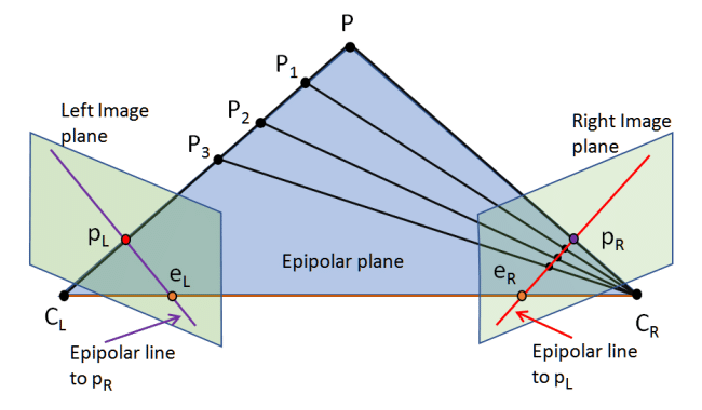
\includegraphics[width=0.9\columnwidth]{figures/epipolar.JPG}
                \caption{\tiny Epipolar geometry \cite{epipolar}}
            \end{figure}
        \end{column}
        \begin{column}{0.4\textwidth}
            \begin{figure}
                \centering
                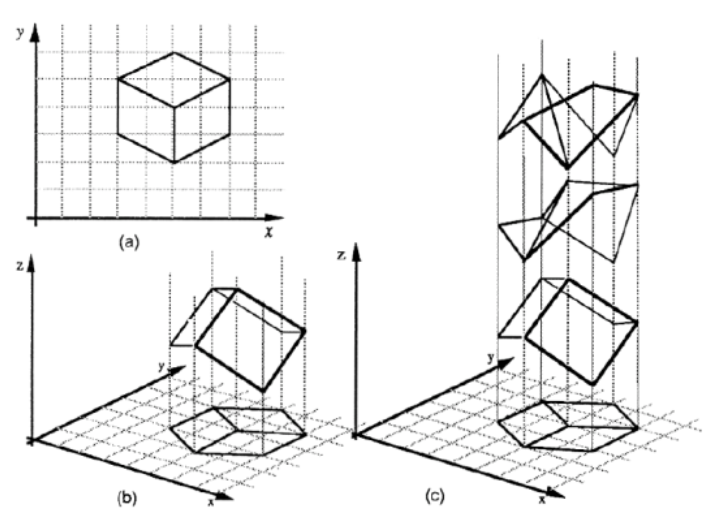
\includegraphics[width=0.85\columnwidth]{figures/ill-posed.PNG}
                \caption{\tiny Many-to-one relationship of 3D scenes and projections \cite{ill-posed}}
            \end{figure}
        \end{column}
    \end{columns}
\end{frame}

\begin{frame}{Monocular Depth Estimation}
    \begin{itemize}
        \item Human perceive depth \tbf{subconsciously}
        \begin{itemize}
            \item Difficult to mathematically describe the process
        \end{itemize}
        \item \tbf{Deep learning} approaches
        \begin{itemize}
            \item \keyword{Supervised} $\rarrow$ Use ground truth depth maps
            \item \tbf{Unsupervised / Semi-supervised} $\rarrow$ Use geometric constraints in video
        \end{itemize}
    \end{itemize}
    
    \begin{figure}
        \centering
        \begin{subfigure}[b]{0.35\textwidth}
            \centering
            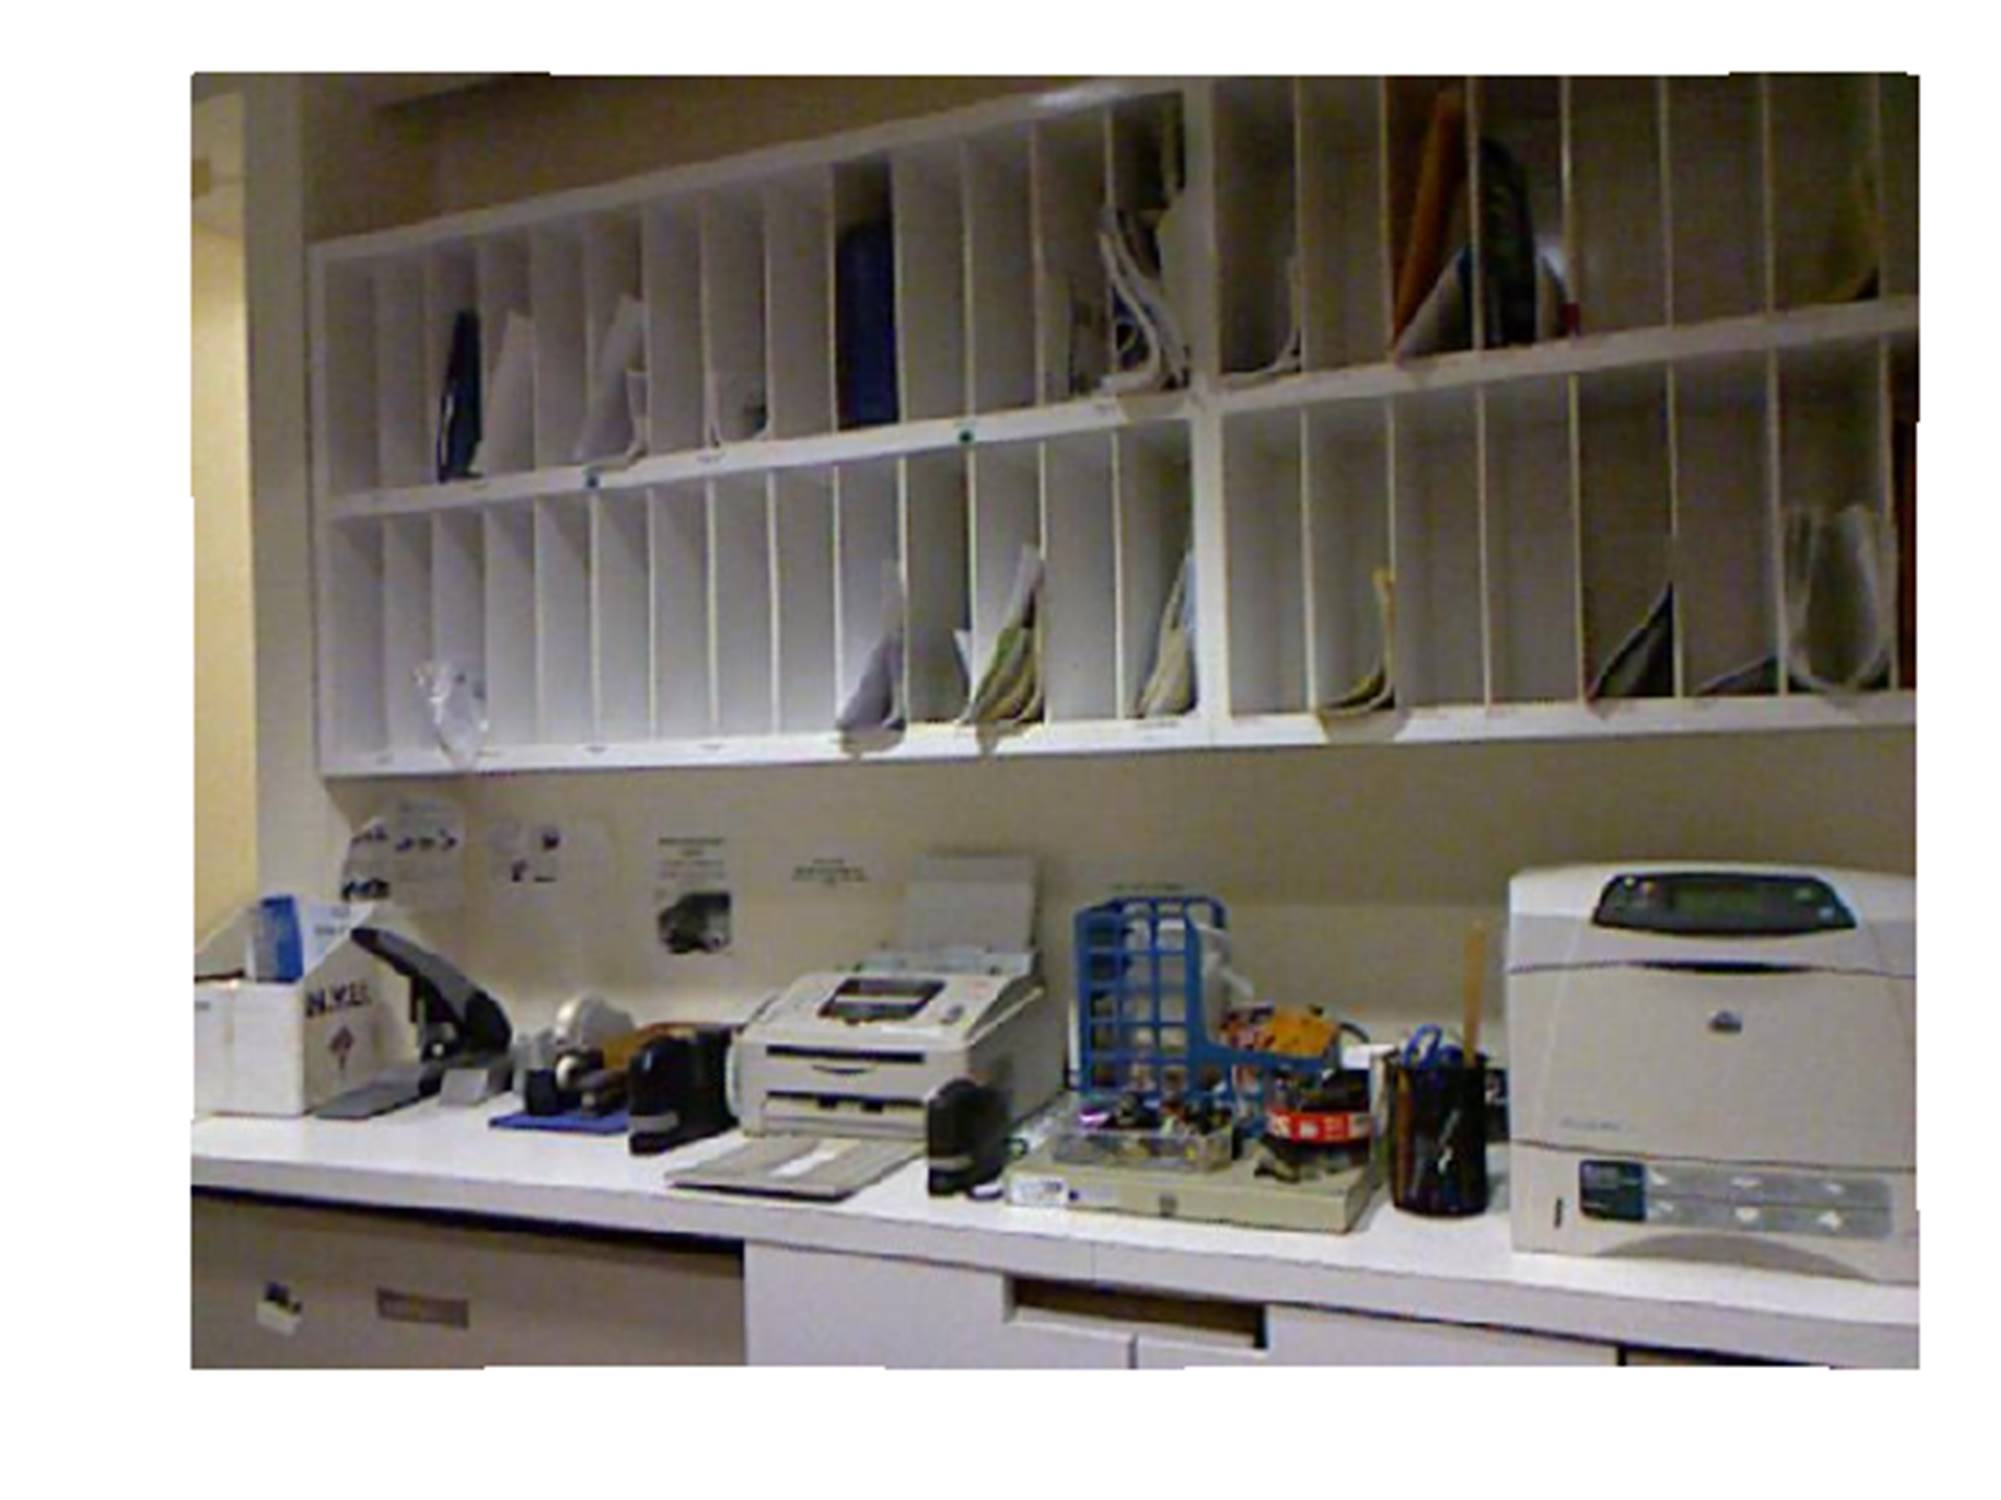
\includegraphics[width=\textwidth]{figures/depthmap_real.jpg}
            \caption{Original RGB image \cite{nyu}}
        \end{subfigure}
        \hspace{2cm}
        \begin{subfigure}[b]{0.35\textwidth}
            \centering
            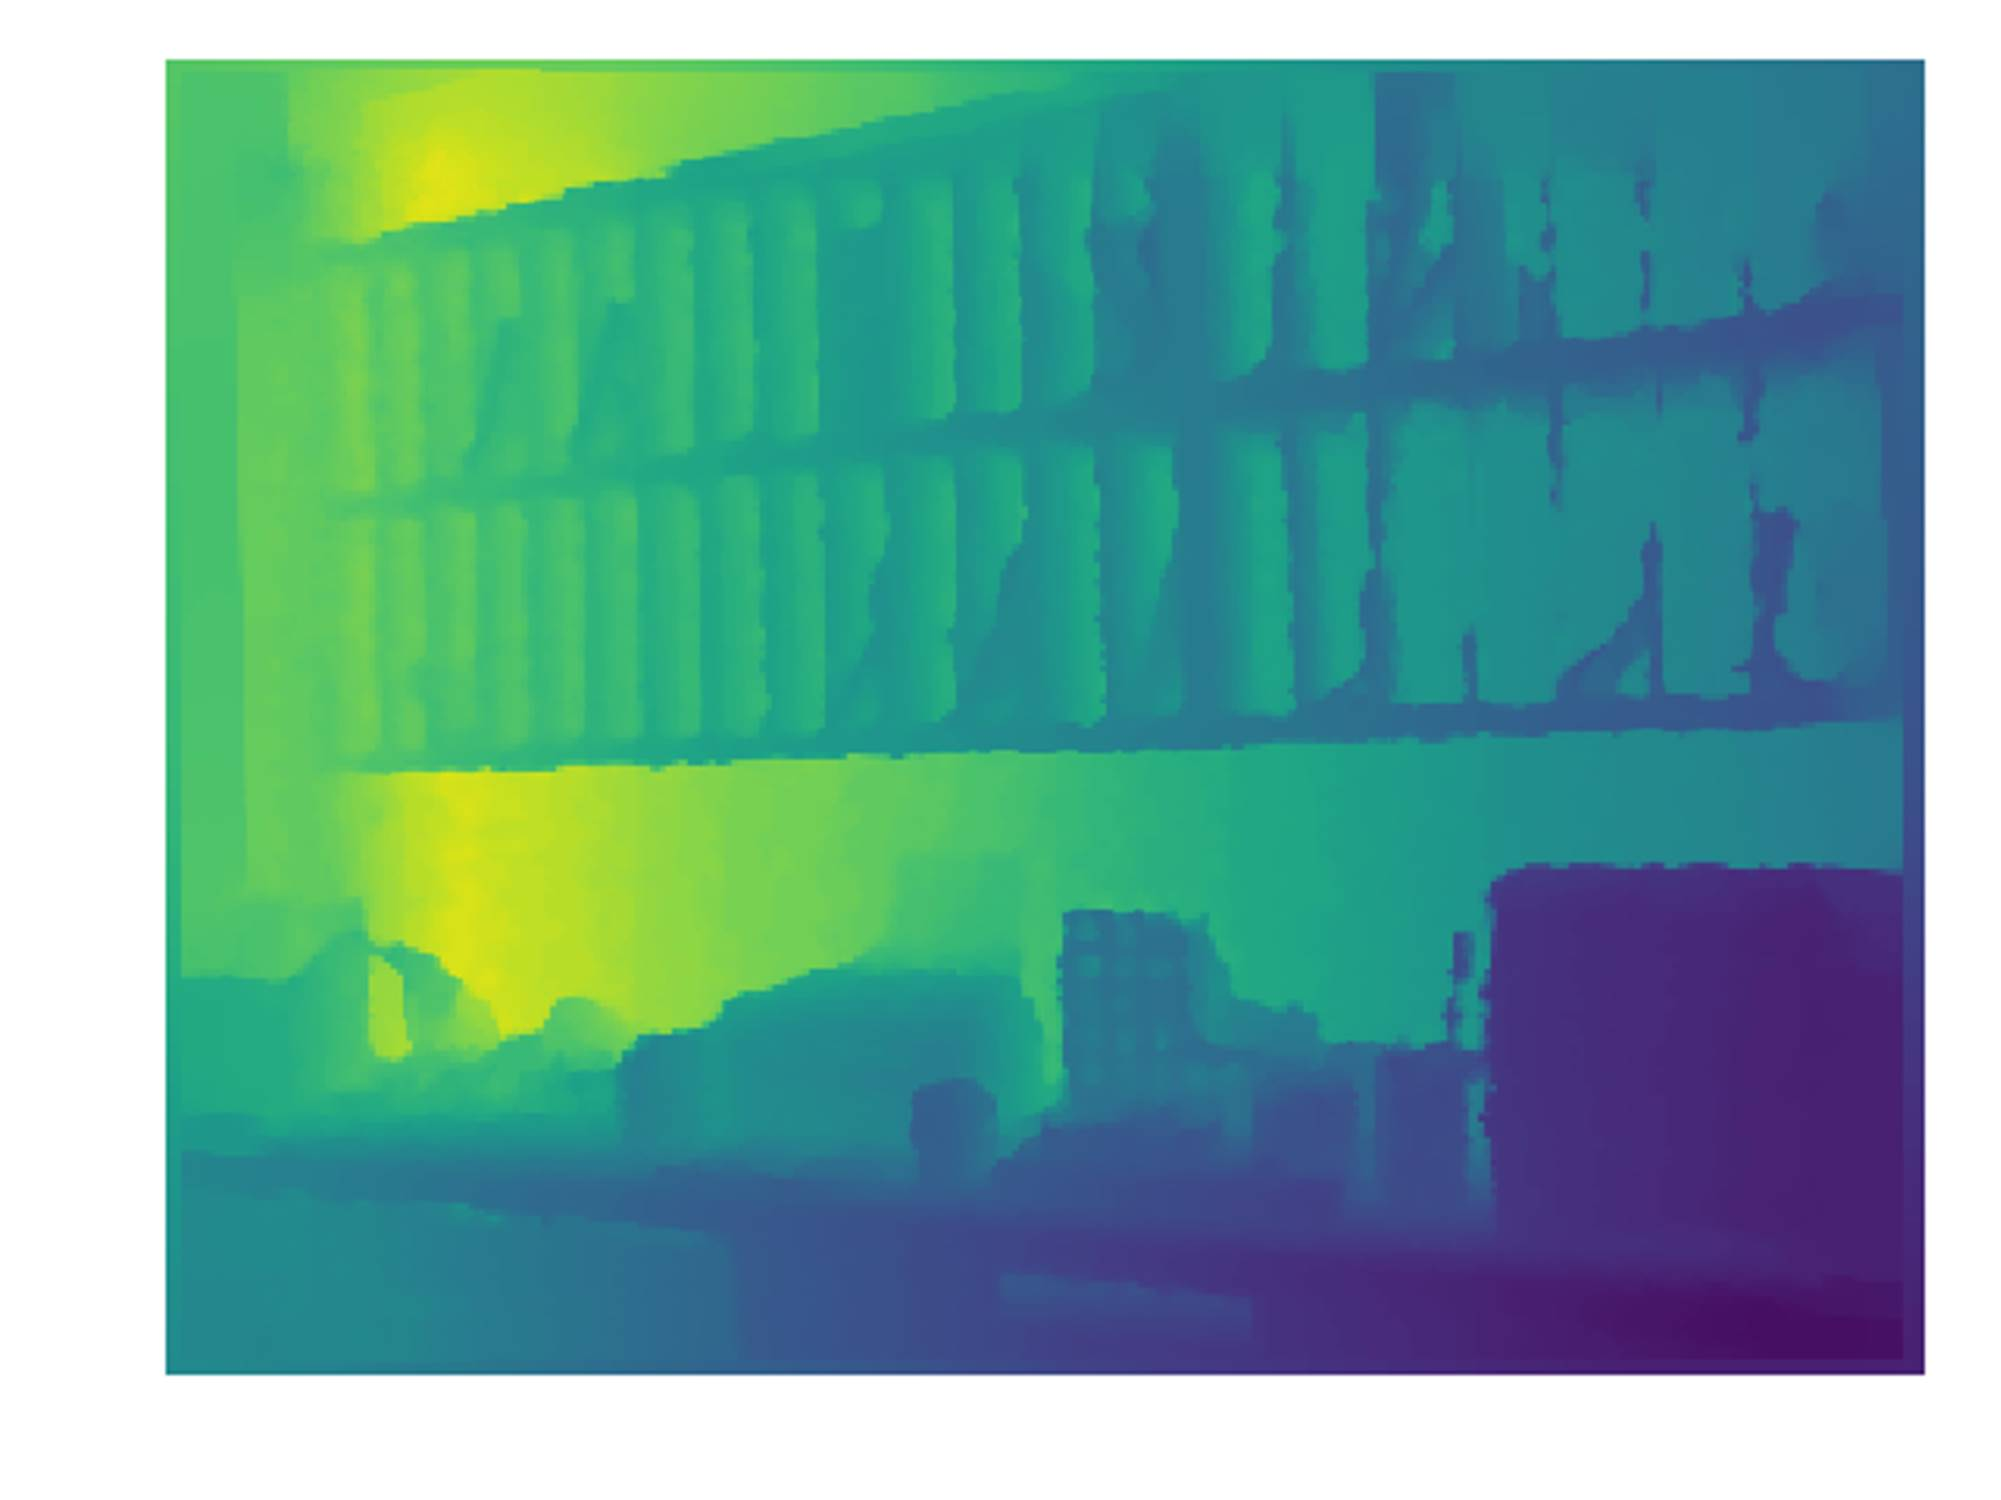
\includegraphics[width=\textwidth]{figures/depthmap_depth.jpg}
            \caption{Corresponding depth map \cite{chaijirawiwat_monocular_2019}}
        \end{subfigure}
    \end{figure}
\end{frame}

\section{Related Works}
\begin{frame}{Related Works}
    \begin{itemize}
        \item \tbf{Monocular Depth Estimation}
        \begin{itemize}
            \item Novel architectures based on \keyword{Convolutional Neural Network (CNN)} or \keyword{Visual Transformer}
            \item \tbf{Multi-tasking} (usually with image segmentation)
            \item \tbf{Domain adaptation}
            \item \tbf{Lightweight Network} for fast inference
            \item and so on...
        \end{itemize}
        \item \tbf{Ensemble Deep Learning}
        \begin{itemize}
            \item Approaches that combine predictions from \keyword{base learners} and generate a better final output (hopefully)
            \item \keyword{Stacked Generalization} linearly combines predictions by using \keyword{meta-learner}
            \item \tbf{While it has been adopted in many tasks, there is no application in monocular depth estimation according to a recent survey} \cite{ensemble_survey}
        \end{itemize}
    \end{itemize}
\end{frame}

\section{Objective}
\begin{frame}{Research Objective}
    \begin{itemize}
        \item Study SG  in monocular depth estimation
        \item Compare performance of different SG setups with \tbf{simple average (baseline)}
    \end{itemize}
    
    \begin{figure}
        \centering
        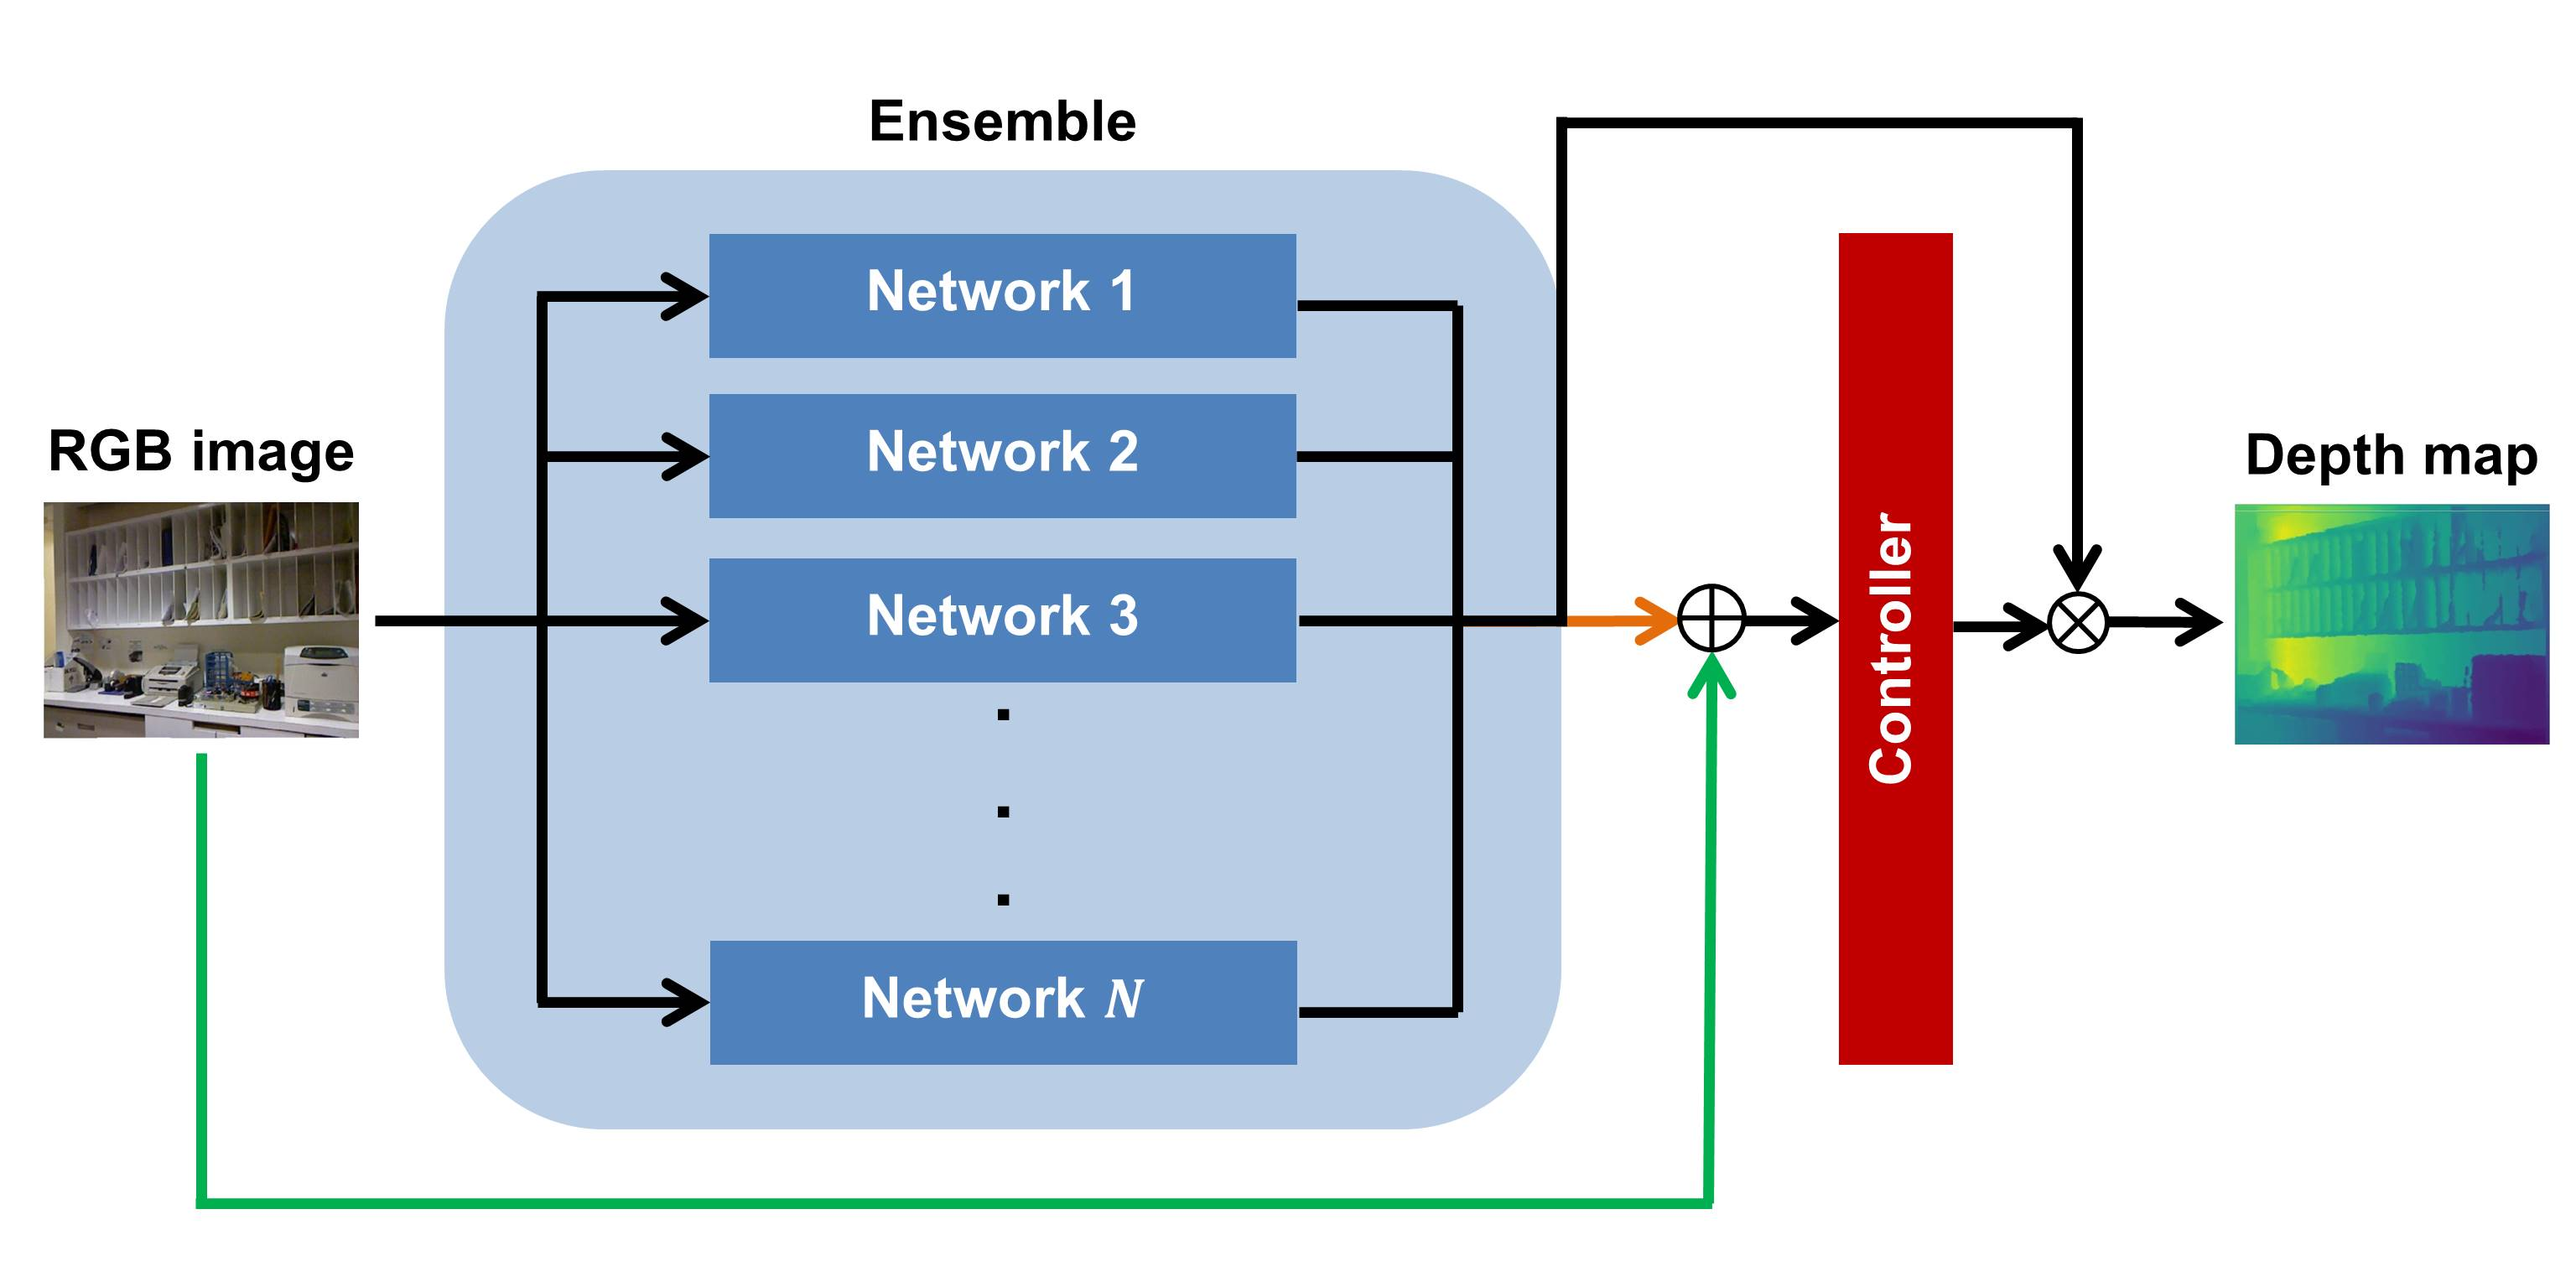
\includegraphics[width=.7\textwidth]{figures/architecture_overview.jpg}
        \caption{Overview of ensemble architecture}
    \end{figure}
\end{frame}

\section{Methodology}
\begin{frame}{Methodology: Base learners}
\begin{itemize}
    \item Adopt 3 SOTAs as base learners
    \begin{itemize}
        \item \keyword{Adabins} \cite{adabins}, \keyword{BTS} \cite{bts}, \keyword{LDRN} \cite{lapdepth}
    \end{itemize}
    \item Every architecture employs \keyword{Encoder-Decoder framework}
    \item Adabins also adds a \tbf{visual transformer} module to learn depth distribution
    \item Input is an \keyword{RGB image} $X \in \Real[H \times W]$. Output is a depth map of the same size.
    
    \vspace{0.2cm}
    \begin{columns}
        \begin{column}{0.5\textwidth}
            \begin{center}
                \subfile{./figures/encoder-decoder}
            \end{center}
        \end{column}
        \begin{column}{0.5\textwidth}
            \begin{center}
                \begin{figure}
                    \centering
                    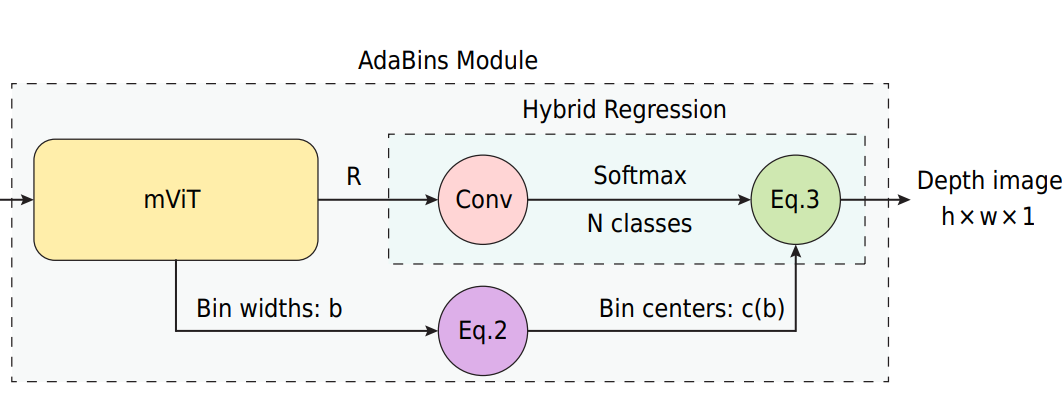
\includegraphics[width=1.0\columnwidth]{figures/adabins.png}
                    \caption{Visual Transformer module in \cite{adabins}}
                \end{figure}
            \end{center}
        \end{column}
    \end{columns}
\end{itemize}
\end{frame}

\begin{frame}{Methodology: Base learners (2)}
    \begin{itemize}
    \item Some modifications to reduce models' size and latency
        \begin{itemize}
            \item Employing \keyword{GhostNet} \cite{ghostnet} as the encoder for all architectures.
            \item Replacing convolution with \keyword{depthwise separable convolution} in \cite{adabins} and \cite{bts} except for atrous convolution layers.
            \item Interpolating \tbf{after} convolution instead of before in \cite{adabins}, as described in \cite{fastdepth}.
        \end{itemize}
    \end{itemize}
    
    \vspace{0.2cm}
    \begin{columns}
        \begin{column}{0.5\textwidth}
            \begin{center}
                \begin{figure}
                    \centering
                    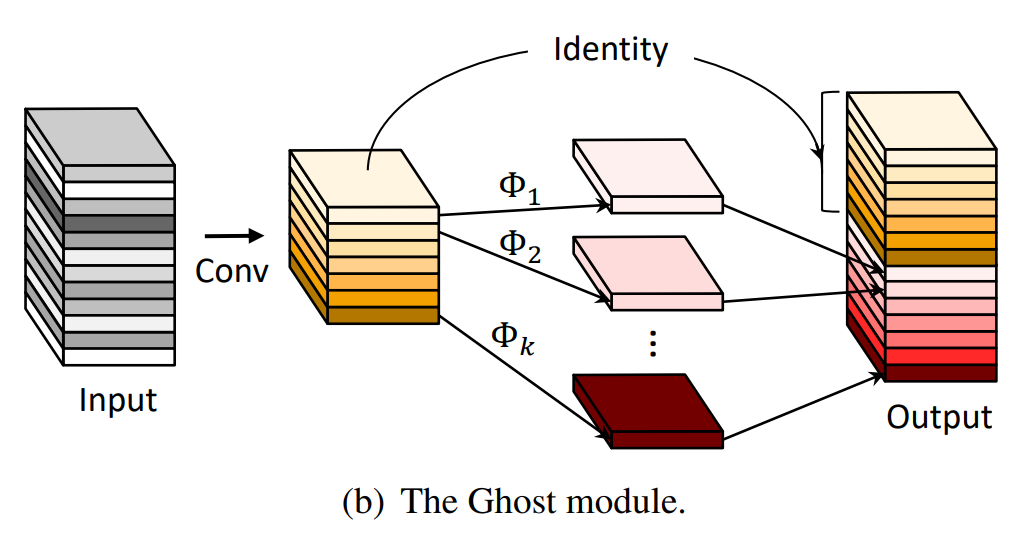
\includegraphics[width=0.9\columnwidth]{figures/ghost_module.png}
                    \caption{Building block of GhostNet \cite{ghostnet}}
                \end{figure}
            \end{center}
        \end{column}
        \begin{column}{0.5\textwidth}
            \begin{center}
                \begin{figure}
                    \centering
                    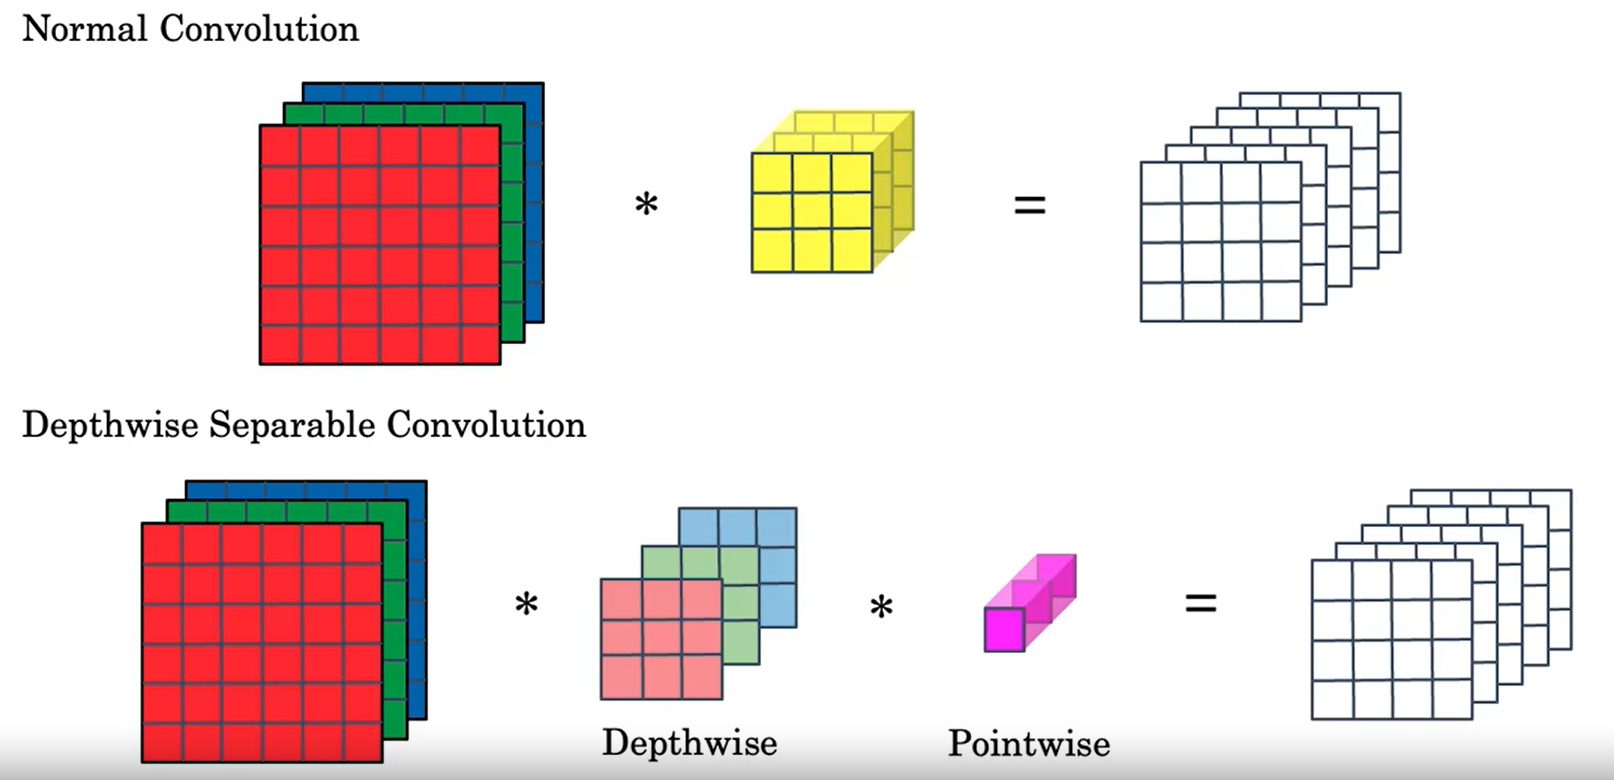
\includegraphics[width=0.9\columnwidth]{figures/DSconv.PNG}
                    \vspace{0.1cm}
                    \caption{Normal convolution and depthwise separable convolution \cite{coursera}}
                \end{figure}
            \end{center}
        \end{column}
    \end{columns}
\end{frame}

\begin{frame}{Methodology: Meta-learner}
\begin{itemize}
    \item For a $N$-ensemble, output is a \keyword{pixel-wise coefficient tensor} $\val[W] \in \Real[N \times H \times W]$
    \item Final prediction $\val[D]^* \in \Real[H \times W]$ is calculated by
    $$
    \val[D]^* = \ssum[i][1][N] \parens*{\val[W] \odot \bracket*{\val[D][1];...;\val[D][N]}^T}(i,:,:)
    $$
    where $\val[D][i]$ is the prediction from $i$-th base learner
    \item Consider 4 design aspects for ablation studies
    \begin{itemize}
        \item Train base learners and controller \tbf{simultaneously} or \tbf{sequentially}?
        \item \tbf{Freeze} base learners' parameters or \tbf{fine-tune} them?
        \item Train with \tbf{RGB images} or \tbf{predictions from base learners}? Or \tbf{both of them}?
        \item Are performance consistent among \tbf{different encoders}?
    \end{itemize}
\end{itemize}

\end{frame}


\begin{frame}{Methodology: Loss Functions}
    \begin{itemize}
        \item \keyword{Pixel-wise depth loss} \cite{eigen2014}
        \begin{itemize}
            \item For mitigating pixel-wise difference in every module
        \end{itemize}
        $$L_{\text{pixel}}=\alpha\sqrt{\frac{1}{N}\sum_{i=1}^{N}y_i^2-\frac{\lambda}{N^2}(\sum_{i=1}^{N}y_i)^2}$$
            where $y_i^{2}=\log(d_i)-\log(d_i^{*})$
        \item \keyword{Bichamfer Loss} \cite{adabins}
        \begin{itemize}
            \item For encouraging distribution of bin centers to follow that of ground truth in \tbf{Adabins} \cite{adabins}
        \end{itemize}
        $$\text{BC}(c(b),D) = \sum_{x \in c(b)} \min_{y \in D} \norm{x-y}_2^2 + \sum_{y \in D} \min_{x \in c(b)} \norm{x-y}_2^2 $$
    \end{itemize}
\end{frame}

\section{Experiment}
\begin{frame}{Experiment}
    \begin{itemize}
        \item Implemented in \keyword{PyTorch} \cite{pytorch} and trained on laboratory server (10 GTX 1080 Ti GPUs) via \keyword{distributed learning}
        \item Employ \keyword{data augmentation} in \cite{adabins} to avoid overfitting
        \item Evaluated on the official split of \keyword{NYU Depth V2 dataset} \cite{nyu} with standard metrics from \cite{eigen2014} 
    \end{itemize}
    \begin{figure}
        \centering
        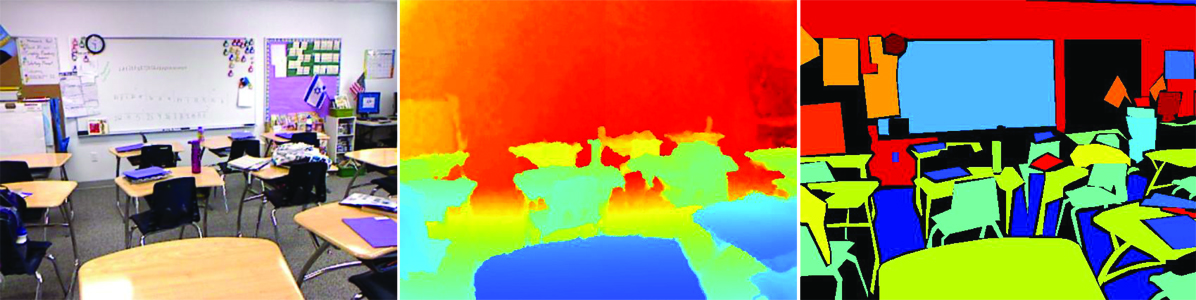
\includegraphics{figures/nyu_sample.jpg}
        \vspace{0.05cm}
        \caption{A sample of raw image, preprocessed depth, and labeled from NYU Depth V2 dataset \cite{nyu}}
    \end{figure}
\end{frame}

\section{Result and Discussion}
\begin{frame}{Result and Discussion}
    \begin{columns}
        \begin{column}{0.35\textwidth}
            \begin{itemize}
                \item Different base learners
                \item Same base learner, same dataset
                \item Same base learner, CV-like dataset
            \end{itemize}
        \end{column}
        \begin{column}{0.65\textwidth}
            \subfile{./tables/baselearner}
        \end{column}
    \end{columns}
\end{frame}

\begin{frame}{Result and Discussion (2)}
    \begin{columns}
        \begin{column}{0.4\textwidth}
            \begin{itemize}
                \item Should train sequentially
                \item Freezing is more stable
                \item Both inputs are better (?)
                \item Performances are consistent (?)
            \end{itemize}
        \end{column}
        \begin{column}{0.6\textwidth}
            \subfile{./tables/metalearner}
        \end{column}
    \end{columns}
\end{frame}

\begin{frame}{Result and Discussion (3)}
    \begin{itemize}
        \item Train base learners \& meta-learner together is fast, but yields worse models
        \begin{itemize}
            \item Need \keyword{hyperparameter tuning} specific to base learners to ensure convergence
            \item Even then, reproducibility is not guaranteed $\rarrow$ inappropriate for practical use
        \end{itemize}
    \end{itemize}
    \begin{figure}
        \centering
        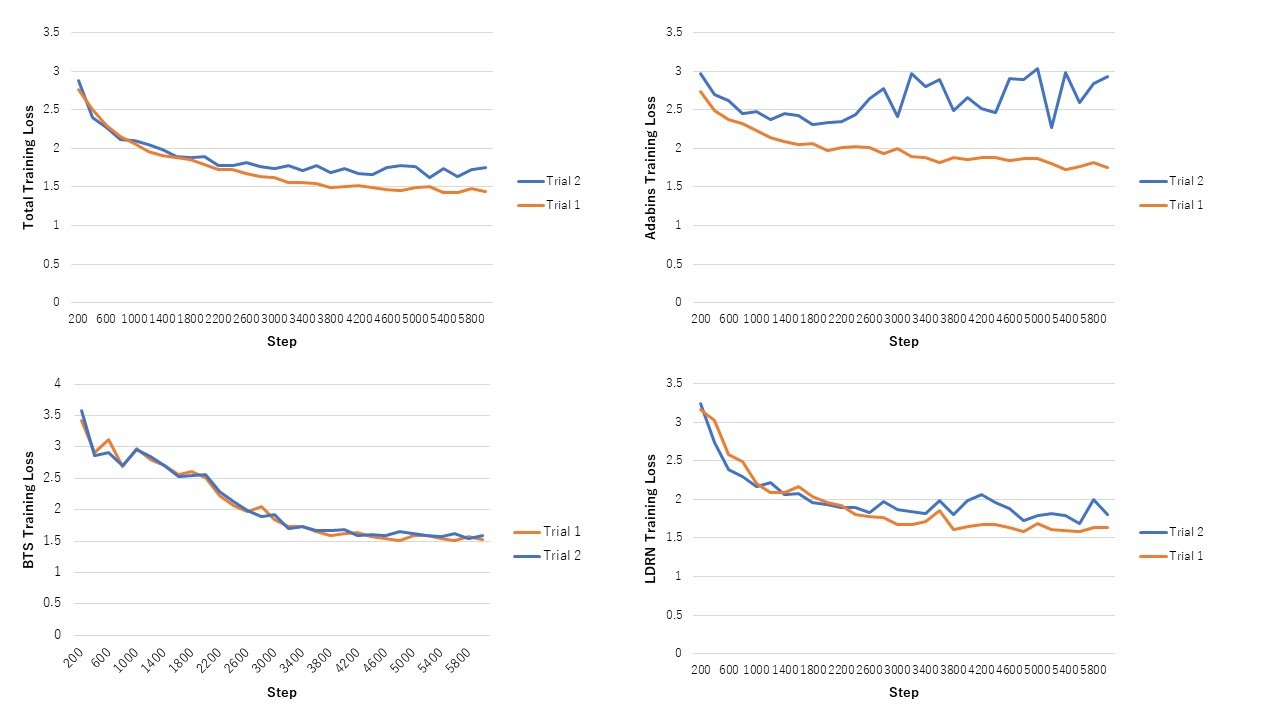
\includegraphics[width=0.575\textwidth]{figures/irp_graph_non-reproducible.jpg}
        \caption{Results are non-reproducible (not even close!)}
    \end{figure}
\end{frame}

\begin{frame}{Result and Discussion (4)}
    \begin{itemize}
        \item Fine-tuning base learners when training meta-learner yields \tbf{training loss fluctuation}
        \item Unfortunately, no improvements in evaluation metrics
    \end{itemize}
    \begin{figure}
        \centering
        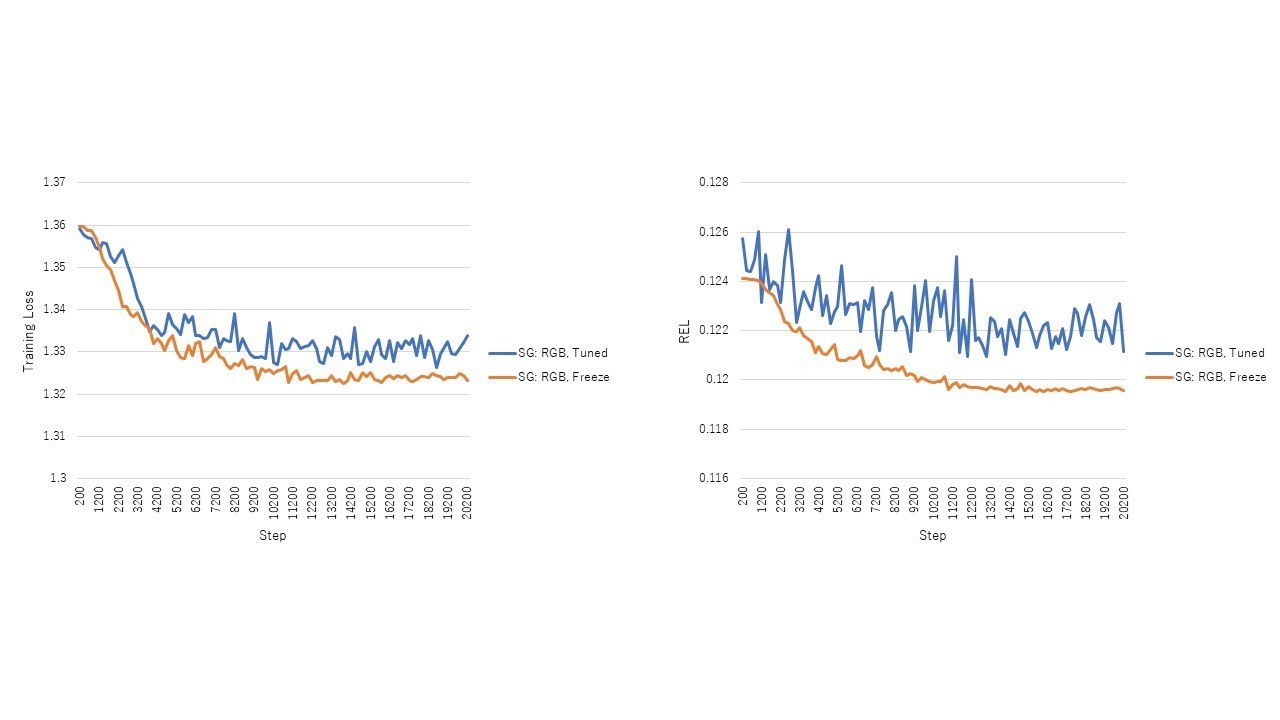
\includegraphics[width=0.9\textwidth,trim={0 {4cm} 0 {4cm}},clip]{figures/irp_graph_fluctuation.jpg}
        \caption{Fluctuations in training loss and an evaluation metric}
    \end{figure}
\end{frame}

\setbeamertemplate{bibliography item}{\insertbiblabel}
\setbeamerfont{bibliography item}{size=\scriptsize}
\setbeamerfont{bibliography entry author}{size=\scriptsize}
\setbeamerfont{bibliography entry title}{size=\scriptsize}
\setbeamerfont{bibliography entry location}{size=\scriptsize}
\setbeamerfont{bibliography entry note}{size=\scriptsize}

\begin{frame}[allowframebreaks, noframenumbering]{References}
    \bibliographystyle{IEEEtran}
    \bibliography{references/figures,
    references/misc,
    references/background-DL,
    references/implementation,
    references/related_depth,
    references/related_ensemble
}
\end{frame}

\appendix

\begin{frame}{Data Augmentation}
    \begin{itemize}
        \item Data augmentation refers to techniques to prevent overfitting by generating more (\tbf{possible}) training examples from original data
        \item Follow data augmentation techniques described in \cite{adabins}:
        \begin{itemize}
            \item \keyword{Random horizontal flipping} with probability of 0.5
            \item \keyword{Random contrast, brightness, and color adjustment} in a range of $[0.9, 1.1]$ with probability of 0.5
            \item \keyword{Random crop}  of size $416 \times 544$
            \item \keyword{Random rotation} of degree in a range of $[-2.5,2.5]$
        \end{itemize}
    \end{itemize}
\end{frame}

\begin{frame}{Evaluation Metrics}
    \begin{itemize}
        \item Follow evaluation metrics described in \cite{eigen2014}:
    \end{itemize}
    \begin{columns}
        \begin{column}{0.4\textwidth}
            $$\func[\text{ThreAcc}]\parens*{\val[\hat{d}], \val[d] ; \delta} = \frac{\abs{S_{\delta}}}{N} \times 100\% $$
            $$\func[\text{REL}]\parens*{\val[\hat{d}], \val[d]} = \frac{1}{N}\ssum[i][1][N]\frac{\abs{\hat{d}_i - d_i}}{d_i} $$
            $$\func[\text{SqREL}]\parens*{\val[\hat{d}], \val[d]} = \frac{1}{N}\ssum[i][1][N]\frac{\norm{\hat{d}_i - d_i}}{d_i} $$
        \end{column}
        \begin{column}{0.6\textwidth}
            $$\func[\text{RMSE}]\parens*{\val[\hat{d}], \val[d]} = \sqrt{\frac{1}{N}\ssum[i][1][N]\parens*{\hat{d}_i - d_i}^2} $$
            $$\func[\text{RMSElog}]\parens*{\val[\hat{d}], \val[d]} = \sqrt{\frac{1}{N}\ssum[i][1][N]\norm{\hat{d}_i - d_i}^2} $$
            $$\func[\text{log10}]\parens*{\val[\hat{d}], \val[d]} = \frac{1}{N}\ssum[i][1][N]\abs{\log_{10}(\hat{d}_i) - \log_{10}(d_i)} $$
        \end{column}
    \end{columns}
    where $S_{\delta} = \cbracket*{d_i | \max\parens*{\frac{\hat{d}_i}{d_i},\frac{d_i}{\hat{d}_i}}<\delta \text{ and } i \leq N}$ and $\delta = 1.25, 1.25^2, 1.25^3$
\end{frame}

\begin{frame}{GhostNet \cite{ghostnet}}
    \begin{itemize}
        \item Based on observation that the output feature maps of convolutional layers often contain much \tbf{redundancy}
        \item Generate some feature maps through usual convolution. Then, apply \keyword{linear operations} to generate more feature maps
        \item \keyword{GhostNet} is ghost modules arranged in a structure similar to \keyword{MobileNetV2}
    \end{itemize}
    \begin{figure}
        \centering
        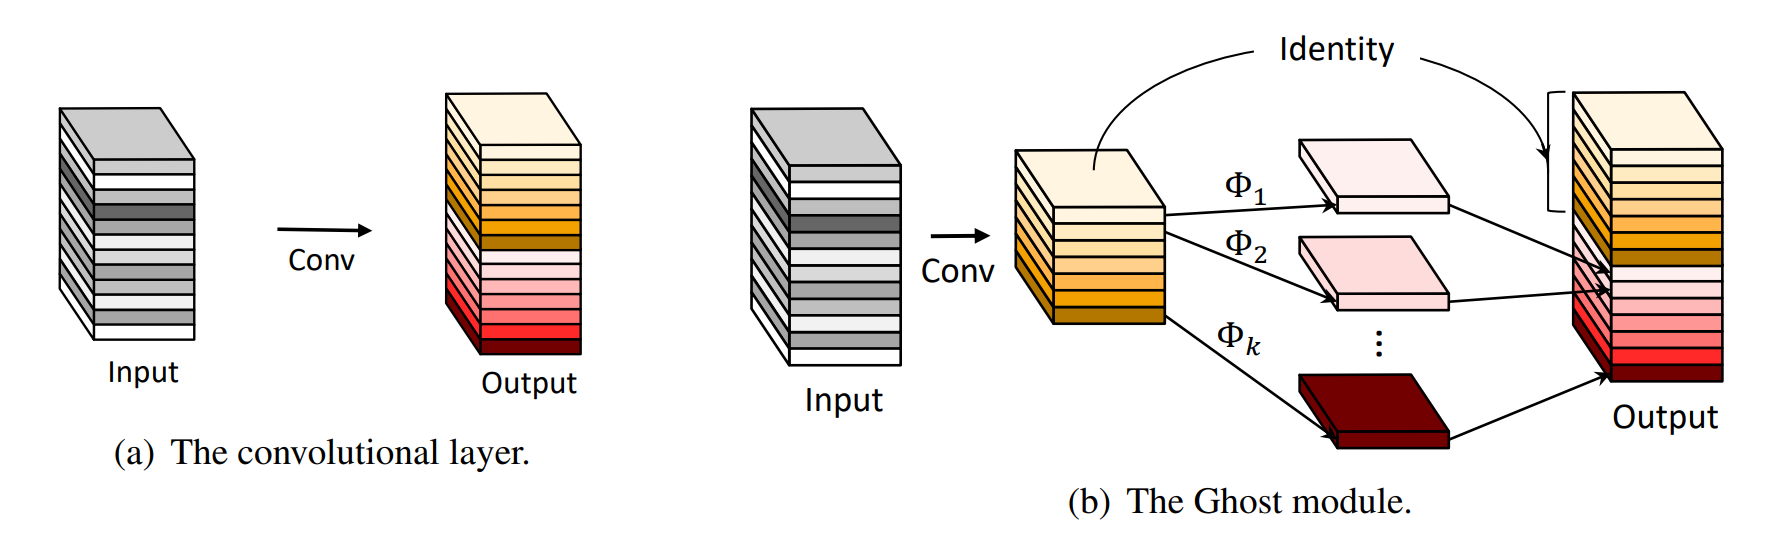
\includegraphics[width=0.8\textwidth]{figures/ghost_net.png}
        \caption{Traditional convolutional layer and The proposed Ghost module \cite{ghostnet}}
    \end{figure}
\end{frame}

\end{document}
